\chapter{Context Survey}
\label{chapter:context}

This section surveys the broader context of the project by reviewing the historical background, key technologies, and recent initiatives that align with the aim of the project. In particular, it examines the Nintendo Wii’s ecosystem, the evolution of its input devices, and the supporting technologies that have enabled both commercial and experimental adaptations.

\section{The Nintendo Wii and its Ecosystem}
Nintendo released the Wii in 2006, quickly earning acclaim for its innovative motion-based controls and engaging game library. Central to its appeal was the Wii Remote (Wiimote), a wireless controller equipped with accelerometers, infrared sensors, and traditional button inputs. These features enabled intuitive, physical interactions, helping to bridge the gap between digital gameplay and physical movement. Over time, the Wii’s local multiplayer format -- often characterised by split-screen or shared-screen experiences -- solidified its reputation as a console focused on communal play. In 2014, Nintendo shut down the Wii’s online services\cite{nintendoTerminationNintendo}, officially ending support for online multiplayer. As a result, third-party solutions, like \textit{Nintendo Wii over IP}, remain the only way to play Wii games online.

\section{Relevant Hardware and Software Technologies}
The project draws on a range of hardware and software technologies to achieve its objectives. Figure~\ref{fig:context_survey} shows a modified version of Figure~\ref{fig:expanded_overview} that highlights where the key technologies fit into the system architecture.


% \vspace{40 mm}
Key technologies include:

\subsubsection{\texttt{WiimoteEmulator}\cite{wiimote_emulator}}
The open-source \texttt{WiimoteEmulator} project on GitHub emulates Wii Remote signals, allowing a real Wii console to interface with a computer acting as an external controller. By replicating the Wiimote’s communication protocol, it lays the groundwork for experimenting with alternative input methods. For this dissertation, I extended a fork of \texttt{WiimoteEmulator} to accept infrared and accelerometer data over a network. This enhancement plays a crucial role in linking remote inputs with local emulation.

\subsubsection{Bluetooth}
Bluetooth is a wireless communication protocol that enables devices to exchange data over short distances.  In the context of this project, Bluetooth facilitates the direct communication between the client machines and the physical Wiimotes as well as between the Wii Remote emulator running on the host machine and the Wii console.

\subsubsection{Raspberry Pi}
The Raspberry Pi serves as a versatile, low-cost computing platform that supports the integration of various peripherals and communication protocols. In this project, both the host and client machines are Raspberry Pi devices. The project uses Raspberry Pi devices due to their Bluetooth capabilities, support for Linux-based operating systems, and prevalence in the hobbyist community. Other platforms, such as the Arduino, ultimately proved unsuitable due to limited processing power and lack of support for the required software libraries.

\subsubsection{\texttt{xwiimote} Library\cite{xwiimote}}
To capture real Wiimote input, the system uses the \texttt{xwiimote} library. Running on a Raspberry Pi, this library interfaces physical Wiimote hardware with software, enabling the system to capture and process motion and button data. A custom Python script then routes this data through the extended emulation system, ensuring correct interpretation of remote control signals.

\begin{figure}[ht]
	\centering
	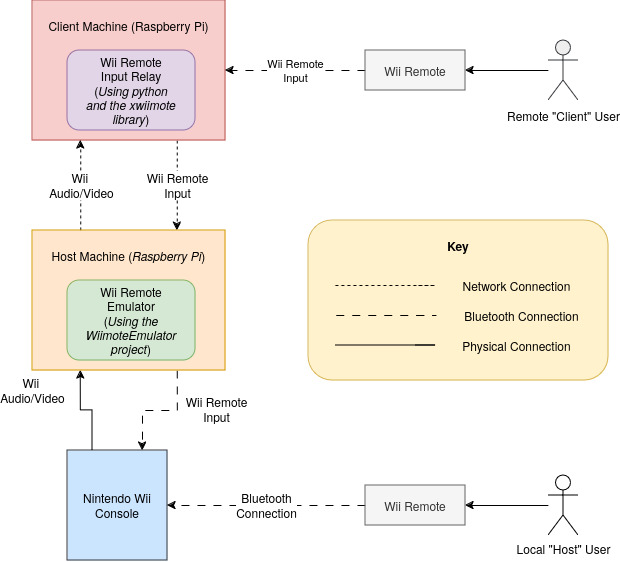
\includegraphics[width=1\textwidth]{context_survey.jpg}
	\caption{Overview of the System with Key Technologies Linked}
	\label{fig:context_survey}
\end{figure}



\section{Recent Work and Similar Endeavours}

The landscape of remote gaming and controller emulation is relatively niche, with few projects addressing the dual challenge of low-latency audiovisual streaming and precise controller input relay. Beyond the core \texttt{WiimoteEmulator} project, the following points are noteworthy:

\subsubsection{Controller Emulation for Legacy Consoles}
Prior research has focused on the emulation of input devices for legacy consoles in order to preserve or extend their operational lifespan. Such projects have enabled modern controllers to interface with older hardware, allowing users to play classic games without original peripherals. For example, the NES Hub utilises the unused expansion port on the NES console to add Bluetooth connectivity, supporting up to four modern wireless controllers without hardware modifications\cite{thevergeWirelessController}. Extending to network-based control -- transmitting sensor data such as IR and accelerometer signals remotely -- is less common and represents a novel contribution of this work.

\subsubsection{Remote Gaming Frameworks}
Advancements in streaming protocols and low latency communication have driven increased interest in remote gaming solutions. Cloud gaming services have transformed gaming by making high-quality games accessible without expensive hardware\cite{cloud_gaming}. Projects like Tailscale transform the ideas of earlier solutions like Hamachi, providing secure, low-latency connections between devices\cite{tailscaleTailscaleHamachi}. However, these solutions are typically designed for modern games and platforms, rather than retro gaming experiences
